\chapter{Resultados} \label{chap:resultados}

También mostrarán capturas de pantalla de cómo se ve en Gazebo el robot y en RViz, ya sea que funcione o no, para el cambio de trayectoria. Describirán lo que ocurre y por qué (si es que saben).

En la primera gráfica se muestra la evolución de la posición en el espacio cartesiano del efector final del robot a lo largo del tiempo. Las curvas representan las componentes X, Y y Z de dicha posición. Esta gráfica permite analizar cómo se desplaza el efector final en el espacio conforme avanzan los segundos de simulación, y verificar que siga la trayectoria deseada. \autoref{fig:cinematicadiferencial}

La segunda gráfica representa la velocidad lineal del efector final en cada una de las tres direcciones espaciales. Las componentes Vx, Vy y Vz indican con qué rapidez cambia la posición en cada eje. Esta información es útil para analizar si el robot está realizando movimientos suaves o si existen cambios bruscos de velocidad. \autoref{fig:cinematicadiferencial}

En la tercera gráfica se observa la aceleración lineal en los ejes X, Y y Z. Esta métrica refleja cómo cambia la velocidad lineal en el tiempo. Picos en esta gráfica podrían indicar esfuerzos mecánicos altos o comportamientos no deseados que podrían comprometer la estabilidad o el control del robot. \autoref{fig:cinematicadiferencial}


\begin{figure}
	\centering
	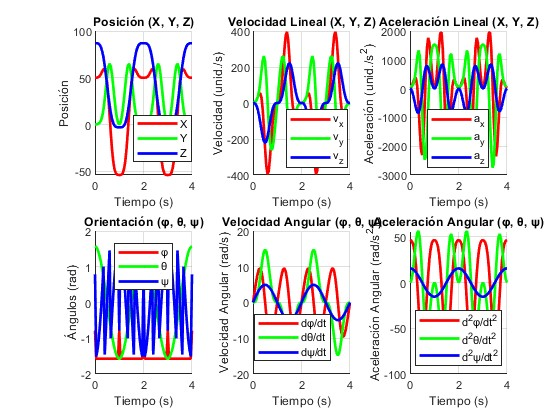
\includegraphics[width=0.5
	\linewidth]{img/cinematicadiferencial}
	\caption{Gráficas Cinemática Diferencial}
	\label{fig:cinematicadiferencial}
\end{figure}

La cuarta gráfica muestra la orientación angular del efector final expresada en términos de los tres ángulos de Euler: phi, theta y psi. Estos ángulos indican cómo rota el efector alrededor de sus propios ejes. Es clave para tareas donde no solo importa la posición, sino también cómo está orientada una herramienta o pinza montada en el extremo. \autoref{fig:cinematicadiferencial}

La quinta gráfica representa la velocidad angular, es decir, qué tan rápido cambian los ángulos de Euler con el tiempo. Se muestran las derivadas respecto al tiempo de phi, theta y psi. Esta gráfica permite verificar si los movimientos rotacionales son suaves y controlados. \autoref{fig:cinematicadiferencial}

Finalmente, la sexta gráfica ilustra la aceleración angular, que es la variación de la velocidad angular. Al igual que con la aceleración lineal, esta información es importante para detectar comportamientos bruscos o posibles problemas de control que afecten la precisión y el rendimiento del robot. \autoref{fig:cinematicadiferencial}

La \autoref{fig:cinematicadirecta}  muestra el resultado de la cinemática directa aplicada a un robot manipulador, representado en un sistema de coordenadas tridimensional con los ejes X, Y y Z. En la gráfica se observa la estructura del robot mediante líneas de color magenta que representan los eslabones conectados por articulaciones. A lo largo de la estructura, se visualizan flechas de colores (rojo, verde y azul) que indican los ejes X, Y y Z locales de cada marco de referencia, los cuales se han obtenido a partir de transformaciones sucesivas conforme a los parámetros del robot. Esta visualización permite comprender la orientación y posición de cada articulación en el espacio. La cinemática directa consiste en calcular la posición y orientación del efector final (la “mano” del robot) a partir de los valores conocidos de las articulaciones, lo cual se refleja en la ubicación final del último eslabón en el espacio tridimensional. En este caso, se puede apreciar que el robot adopta una configuración en forma de “L” invertida, lo que sugiere una posible estructura tipo SCARA o un brazo articulado con varios grados de libertad. El resultado gráfico proporciona una representación clara del comportamiento espacial del robot y permite validar que los cálculos de la cinemática directa han sido correctamente implementados.

\begin{figure}
	\centering
	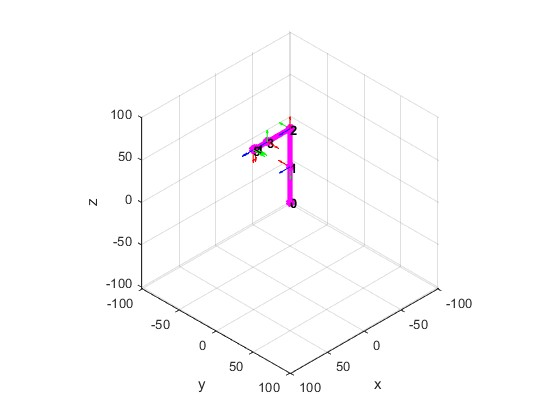
\includegraphics[width=0.5\linewidth]{img/cinematicadirecta}
	\caption{Cinemática Directa}
	\label{fig:cinematicadirecta}
\end{figure}

En la \autoref{fig:ros1}  se observa un brazo robótico en una postura extendida, visualizado mediante RViz, herramienta del entorno ROS. Aunque no se muestran marcas explícitas de la trayectoria, se puede inferir su recorrido a partir de la configuración actual del robot. La trayectoria seguida por el efector final parece haber sido descendente y hacia adelante, lo cual es común en tareas de manipulación de objetos. Es probable que el robot haya iniciado desde una posición más elevada y replegada, para luego extender sus eslabones intermedios, desplazando el efector final en la dirección frontal (eje X positivo) y descendiendo gradualmente hacia una posición más baja (eje Z negativo). La orientación final del efector, apuntando hacia abajo, sugiere que el robot se encuentra listo para interactuar con el entorno, ya sea para tomar un objeto, realizar un ensamble o ejecutar una acción específica. Esta trayectoria implica un movimiento controlado y suave en el plano XZ, característico de movimientos precisos y planificados mediante algoritmos de planificación de trayectorias y control cinemático. En la \autoref{fig:sistemadecoordenadassw} se puede ver el sistema de coordenadas del robot.

\begin{figure}
	\centering
	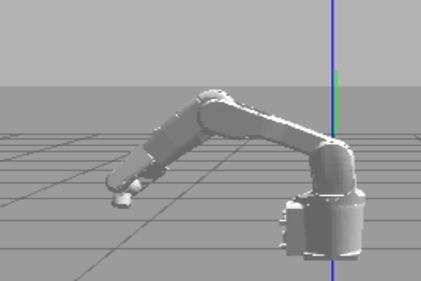
\includegraphics[width=0.5\linewidth]{img/ROS1}
	\caption{RViz del Robot}
	\label{fig:ros1}
\end{figure}

\begin{figure}
	\centering
	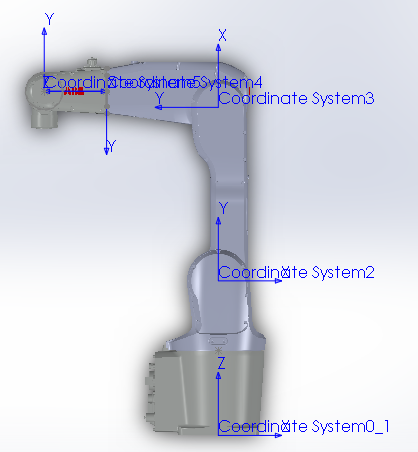
\includegraphics[width=0.3\linewidth]{img/SISTEMADECOORDENADASSW}
	\caption{Sistema de Coordenadas}
	\label{fig:sistemadecoordenadassw}
\end{figure}



